\vspace{-1ex}
\epigraph{``We cannot solve our problems with the same thinking we used when we created them!"}{--- \textup{Attributed to Albert Einstein}}
\vspace{-2ex}

\vspace{-3ex}
\section{Introduction}\label{sec:intro}
For decades, AI research has focused on designing machine learning algorithms that learn from data~\citep{pitts1943linear, mcculloch1949brain, mcculloch1948statistical, samuel1959some} or experience~\citep{silver2025welcome, sutton1998reinforcement, Robotica_1999}; often by optimizing an objective $\mathcal{L}(\boldsymbol{\theta})$ over parameters  $\boldsymbol{\theta} \in \Theta$ with gradient-based methods. While traditional machine learning techniques required careful engineering and domain expertise to design feature extractors, limiting their ability to directly process and learn from natural data~\citep{lecun2015deep}, deep representation learning offered a fully automated alternative to discover the representations needed for the task. Thereafter, deep learning has been an inseparable part of the large-scale computational models with seminal success in chemistry and biology~\citep{jumper2021highly}, games~\citep{silver2016mastering, silver2018general}, computer vision~\citep{krizhevsky2012imagenet, dosovitskiy2021an}, and multimodal and natural language understanding~\citep{comanici2025gemini, liu2024deepseek, achiam2023gpt}.   


\begin{figure*}
    \centering
    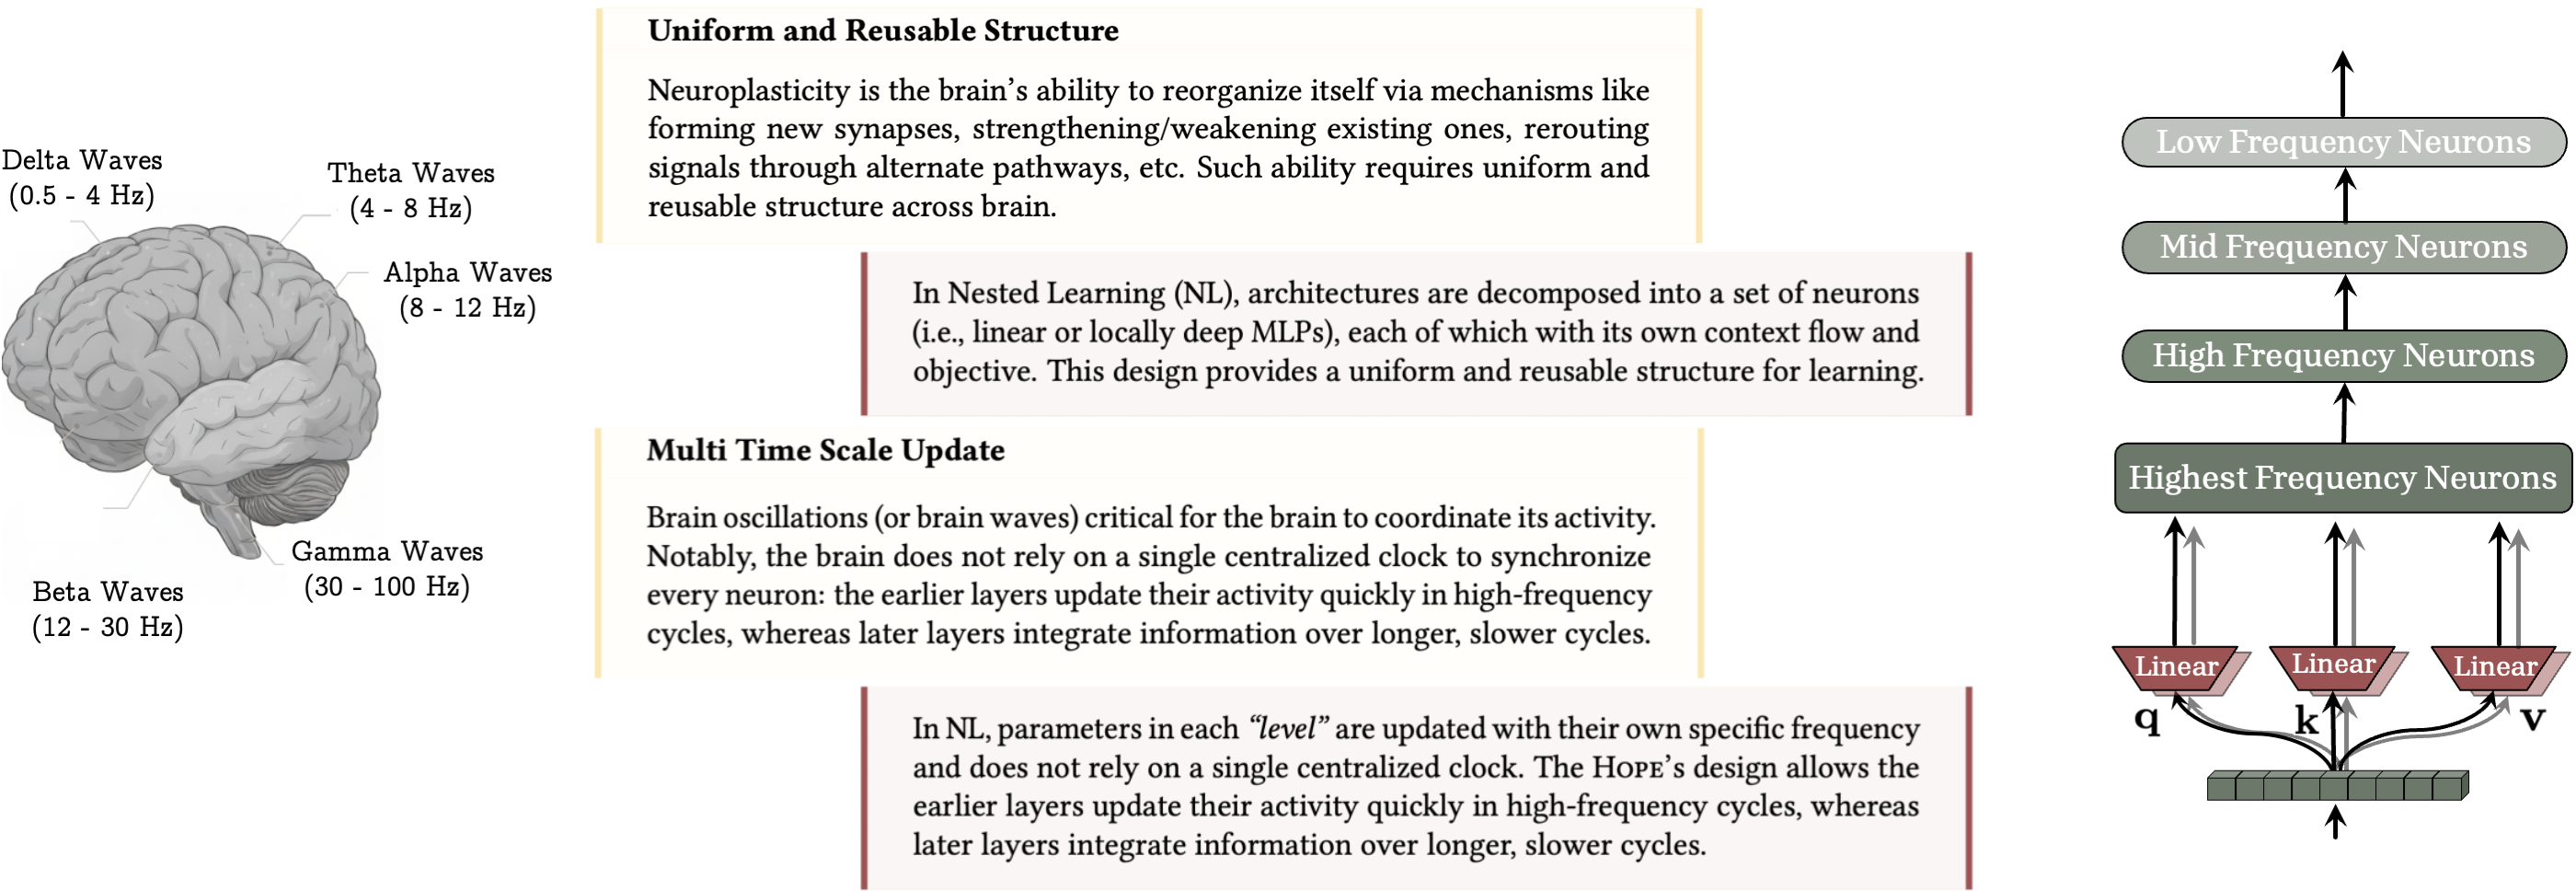
\includegraphics[width=\linewidth]{Images/NL_teaser.png}
    \caption{The uniform and reusable structure as well as multi time scale update in the brain are the key components to unlock the continual learning in humans. Nested Learning (NL) allows for multi time-scale update for each component of the brain, while showing that well-known architectures such as Transformers are in fact linear layers with different frequency updates.}
    \label{fig:NestedLearning_teaser}
\end{figure*}


Stacking of multiple layers, as it is done in deep learning models, provides the models with better expressive power in representing complex features, and more internal computations (e.g., \#FLOPS)~\citep{montufar2014number, poole2016exponential, hestness2017deep}, all of which are critical and desirable characteristics for static tasks that require in-distribution predictions over an a-priori fixed set. This deep design, however, is not a universal solution to all the challenges and cannot help the expressive power of the models in multiple aspects, for example: (i) The computational depth of deep models might not change with more layers~\citep{merrill2022saturated, sanford2024transformers}, leaving their ability to implement complex algorithms untouched compared to traditional shallow approaches~\citep{merrill2024the}; (ii) The capacity of some class of parameters might show marginal improvement with increasing the depth/width of the model~\citep{kaplan2020scaling}; (iii) The training process might converge to a suboptimal solution, mainly due to the suboptimal choice of the optimizer or its hyperparameters; and (iv) The model's ability to fast adapt to a new task, continually learn, and/or generalize to out-of-distribution data might not change with stacking more layers and requires more careful designs. 

The core part of the efforts to overcome the above challenges and to enhance the capability of deep learning models concentrate on: (1) developing more expressive class of parameters (i.e., neural architectures)~\citep{LSTM, fukushima1980neocognitron, transformers, krizhevsky2012imagenet, behrouz2024titans}; (2) introducing objectives that can better model the tasks~\citep{rumelhart1986learning, goodfellow2020generative, alshammari2025unifying, kingma2014autoencoding, hjelm2018learning};  (3) designing more efficient/effective optimization algorithms to find better solutions or with more resilience to forgetting~\citep{kingma2014adam, jordanmuon, gupta2018shampoo, farajtabar2020orthogonal}; and (4) scaling the model size to enhance its expressivity, when the ``right'' choice of architecture, objective, and optimization algorithms are made~\citep{hoffmann2022training, brown2020language, kaplan2020scaling}. Collectively, these advancements and new findings on scaling patterns of deep models have established the foundations upon which Large Language Models (LLMs) have been built.


The development of LLMs marks a pivotal milestone in deep learning research: a paradigm shift from task-specific models to more general-purpose systems with various emergent capabilities as a result of scaling the ``right'' architectures~\citep{brown2020language, schaeffer2023emergent}. Despite all their success and remarkable capabilities in diverse sets of tasks~\citep{comanici2025gemini, nijkamp2023codegen, wang2023visionllm}, LLMs are largely static after their initial deployment phase, meaning that they successfully perform tasks learned during pre- or post-training, but are unable to continually acquire new capabilities beyond their immediate context. The only adaptable component of LLMs is their \emph{in-context learning} ability–a (known to be emergent)~characteristic of LLMs that enables fast adaption to the context and so perform zero- or few-shot tasks~\citep{brown2020language}. Beyond in-context learning, recent efforts to overcome the static nature of LLMs either are computationally expensive, require external components, lack generalization, and/or might suffer from catastrophic forgetting~\citep{eyuboglu2025cartridges, yu2025finemedlmo, akyureksurprising}, which has led researchers to question if there is a need to revisit how to design machine learning models and if a new learning paradigm beyond stacking of layers is required to unleash the capabilities of LLMs in continual setups. 





\head{Current Models only Experience the Immediate Present}
As an analogy and to better illustrate the static nature of LLMs, we use the example of anterograde amnesia–a neurological condition where a person cannot form new long-term memories after the onset of the disorder, while existing memories remain intact~\citep{scoville1957loss}. This condition limits the person's knowledge and experiences to a short window of present and long past–before the onset of the disorder–which results in continuously experiencing the immediate present as if it were always new. The memory processing system of current LLMs suffer from a similar pattern. Their knowledge is limited to either, the immediate context that fits into their context window, or the knowledge in MLPs that stores long-past, before the onset of \emph{``end of pre-training.''} This analogy, has motivated us to take inspiration from neurophysiology literature and how~brain~consolidate~its~short-term~memories.






 

\subsection{Human Brain Perspective and Neurophysiological Motivation}\label{sec:brain-perspective}
Human brain is highly efficient and effective when it comes to continual learning, which is often attributed to neuroplasticity—the brain's remarkable capacity to change itself in response to new experiences, memories, learning, and even damage~\citep{pascual2005plastic, johnston2009plasticity}. Recent studies support that the formation of Long-term memory involves at least two distinct but complementary consolidation processes~\citep{Stepwise-consolidation2021, frey1997synaptic, yang2024selection}: (1) A rapid ``online'' consolidation (also known as synaptic consolidation) phase occurs immediately or soon after learning, even during wakefulness. This is when new and initially fragile memory traces are stabilized and begin transferring from short-term to long-term storage; (2) An ``offline'' consolidation (also known as systems consolidation) process repeats the replay of the recently encoded patterns—during sharp‑wave ripples (SWRs) in the hippocampus, coordinated with cortical sleep spindles and slow oscillations—strengthens and reorganizes the memory and supports transfer to cortical sites~\citep{ji2007coordinated, peyrache2009replay, foster2006reverse}. 


Coming back to the analogy of anterograde amnesia, evidence indicates that the condition can impact both stages, but especially the online consolidation phase, mainly due to the fact that hippocampus is the gateway for encoding new declarative memories, and so its damage means new information never will be stored in long-term memory. As mentioned above, the design of LLMs, and more specifically Transformer-based backbones, suffers from a similar condition after the pre-training phase. That is, the information provided in the context, never impacts the long-term memory parameters (e.g., feedforward layers), and so the model is not capable of acquiring new knowledge or skill, unless the information is still stored in the short-term memory (e.g., in-context or attention). To this end, although the second stage is equally, or even more, crucial for the consolidation of memories, and its absence can damage the process and might cause loss of memory~\citep{drummond2000altered, yoo2007deficit}, in this work, we focus on the first stage: memory consolidation as an online process. As discussed earlier, the memory processing, its online consolidation, and so continual learning ability of humans are known to be highly relied on the neuroplasticity as well as neural oscillations~\citep{bliss1993synaptic, buzsaki2004neuronal, klinzing2019mechanisms}.




\head{Multi Time scale Processing System} Brain oscillations (also known as brainwaves)–a rhythmic fluctuations in brain activity–is not mere byproducts of brain function but is increasingly understood to play a crucial role in various cognitive functions such as attention, memory, and decision-making, and to be a core mechanism for organizing neural computation, coordinating communication between brain regions, and gating the synaptic plasticity that underlies learning and memory ~\citep{fries2015rhythms, fell2011role, cavanagh2014frontal}. These brainwaves are the results of the brain coordinating its computations in different timescales and frequency updates, where each frequency determines how often groups of brain neurons become active and share updated information.
More specifically, such neural oscillations are typically categorized into distinct frequencies, each of which has been associated with different cognitive functions and, critically, different timescales of information processing: ranging from (1) fast Gamma waves (frequency of $30$-$150$ Hz) that are mainly associated with sensory information to (2) Beta waves (frequency of $13$ - $30$ Hz) that are mainly associated with active thinking~\citep{buzsaki2004neuronal,BuschmanMiller2007Science,Lundqvist2016Neuron}, and (3) slow Delta and Theta waves (frequency of $0.5$ - $8$ Hz), mainly responsible for memory consolidation and learning~\citep{DiekelmannBorn2010NRN,Marshall2006Nature,Ngo2013Neuron,Staresina2015NatNeuro,Heusser2016NatNeuro,Daume2024Nature}. 

In deep learning models, however, the weights of the architectures are fixed at test time and also it is common in pre-training to use the same update rate for all the blocks/layers in the model. Later, in \autoref{sec:revisit}, however, we show that in-context learning provides an extreme case of this design and in fact, Transformer architectures are based on two extreme frequencies of update: i.e., $\infty$ and $0$ for attention and MLP blocks, respectively.   








\head{Brain's Uniform and Reusable Structure} As discussed earlier, neuroplasticity is the brain's remarkable capability to change itself in response to new memories, knowledge, and even damage~\citep{pascual2005plastic, johnston2009plasticity}. This characteristic suggests a uniform architecture where neural elements are not rigidly dedicated to one function but are instead reusable, capable of being flexibly redeployed to support different cognitive needs. One real-world example of neural reusability is hemispherectomy–the surgical removal or disabling of one cerebral hemisphere, usually to alleviate severe epilepsy. Amazingly, if this surgery is done in childhood, patients can lead largely normal lives into adulthood with high functioning cognition and intact neural network organization that contains all the same core brain networks present in a typical two-hemisphere brain (networks for language, vision, etc.). This extraordinary outcome provides real-life proof of the brain’s uniform architecture. That is, even half a brain can reallocate resources and reorganize so that the person can function extremely well. Such cases, along with documented instances of individuals living relatively normally with missing pieces of cortex, highlight the brain's uniform and reusable structure.


Furthermore, this interpretation of brain's uniform and reusable structure demonstrate that memory in human brain is not an isolated system in some specific areas, and mainly is distributed across brain. That is, contrary to the traditional models of memory that often implied that different types of memory reside in distinct brain structures (e.g. short-term memory in frontal cortex vs. long-term memory in the hippocampus and cortex), modern research advocate for distributed neural circuits memory processing across multiple regions~\citep{christophel2017distributed, roy2022brain, kitamura2017engrams}. 


The modern deep learning architectures in recent years, however, at least on the surface, seem to be heterogeneous and are based on a combination of a subset of self-attention variants~\citep{transformers}, modern recurrent neural networks~\citep{katharopoulos2020transformers, schlag2021linear, peng2025rwkv7, behrouz2024titans}, canon layers~\citep{Allenzhu2025-canon}, global convolutions~\citep{poli2023hyena, hasani2023liquid}, and MLP blocks~\citep{shazeer2020glu}. This raises the question of whether we need a new uniform architecture, or if our beliefs about the heterogeneity of current models need to be revisited.




\begin{figure*}
    \centering
    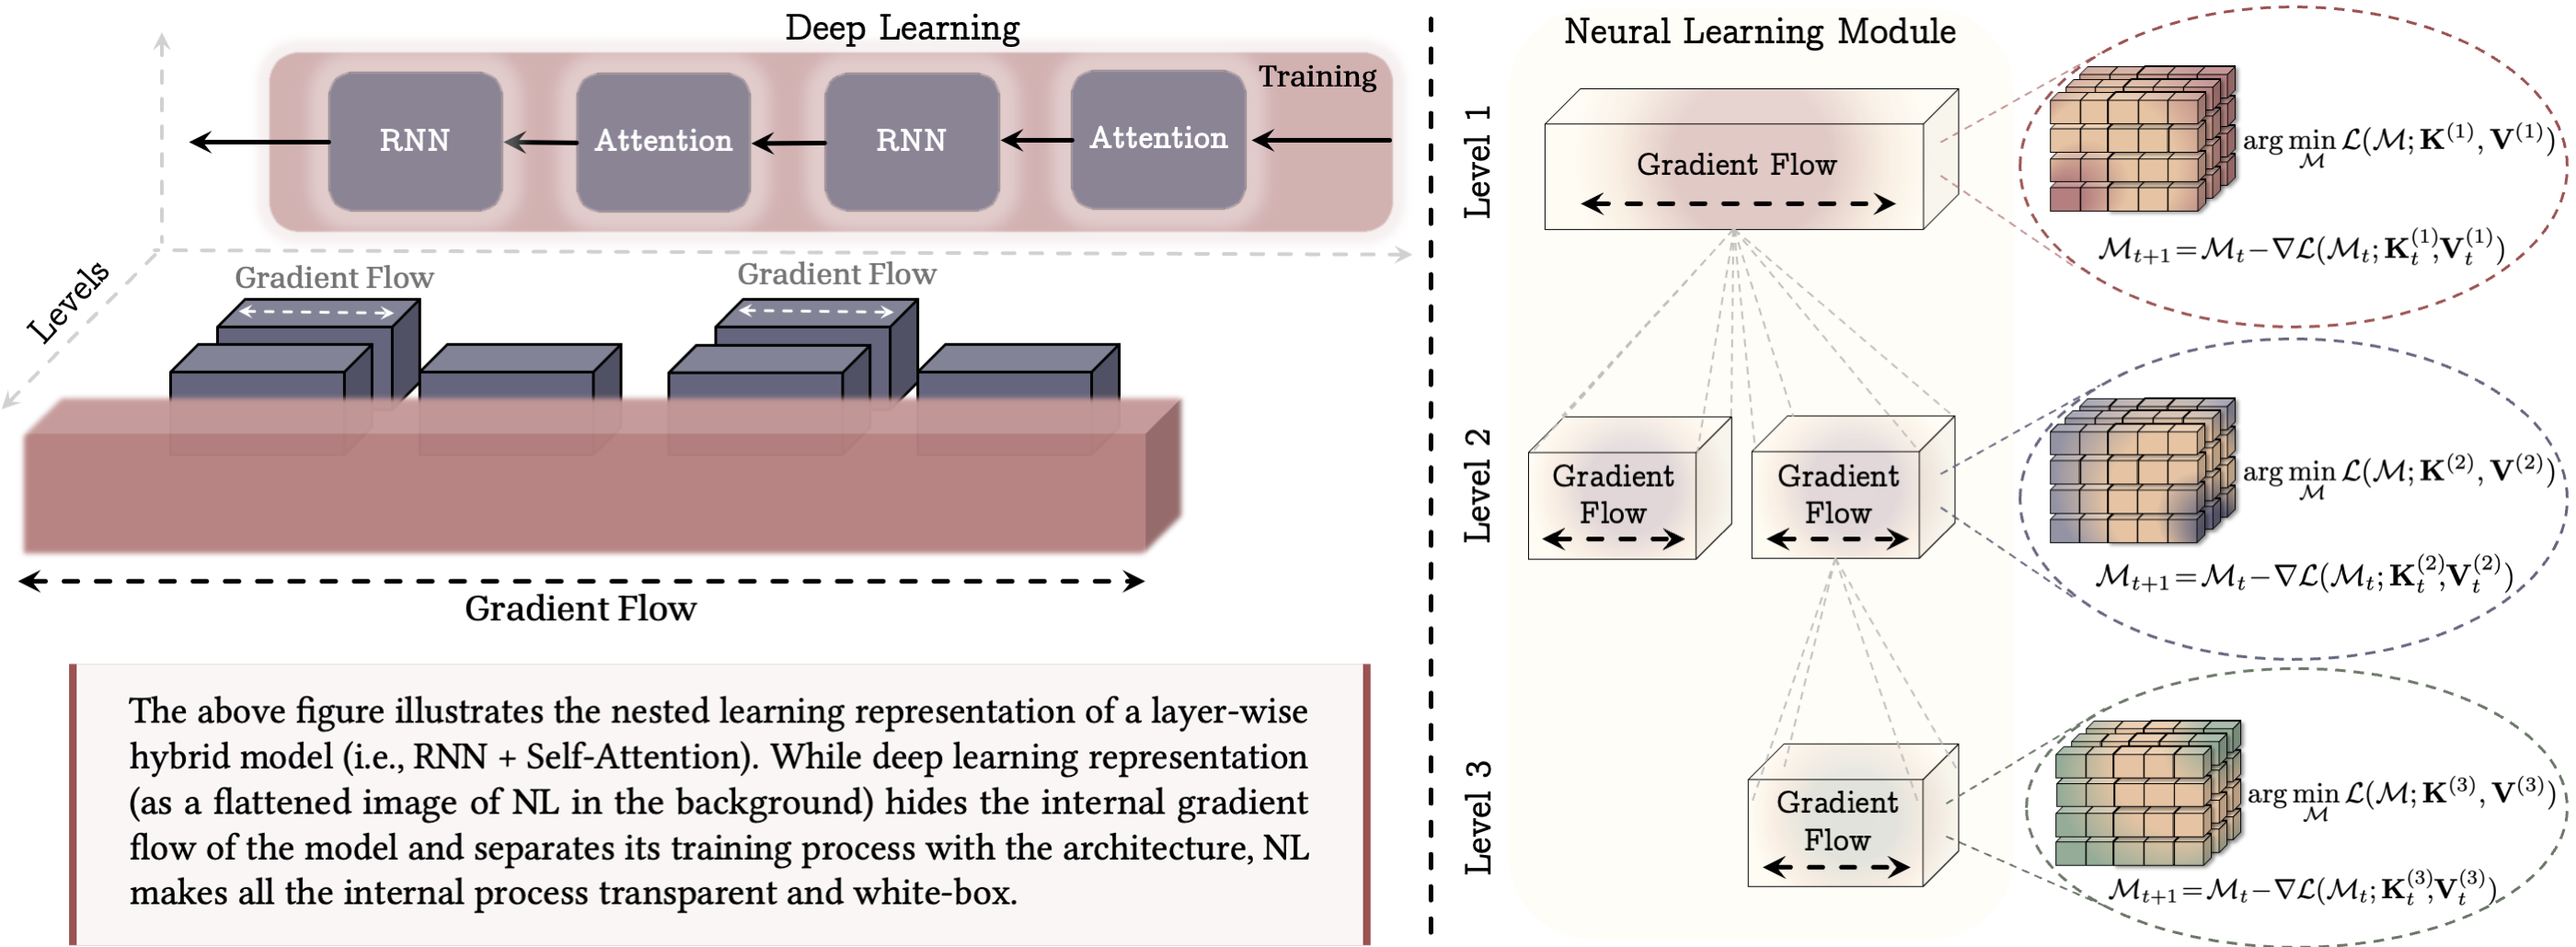
\includegraphics[width=\linewidth]{Images/Nested_main.png}
    \vspace{1ex}
    \caption{Nested Learning Paradigm that represent a machine learning model and its training procedure as a set of nested optimization problems. (\textbf{Left}) An example of Hybrid architecture. While deep learning perspective, as the flattened image of NL, does not provide insight about the depth of computation in the blocks, NL transparently represent all the inner gradient flows. (\textbf{Right}) A Neural Learning Module: A computational model that learns how to compress its own context flow. For example, the first level corresponds to the model's most outer-loop training, often~refer~to~as~``\emph{pre-training}''~step.}
    \label{fig:NestedLearning}
\end{figure*}


\subsection{Contributions and Roadmap}
In this paper, we aim to present a unifying learning paradigm that not only provides new insights about existing algorithms, methods, and architectures, but it also reveals a new dimension to stacking layers in deep learning with enhancement of the computational depth, and continual learning ability of models. After discussing preliminary concepts and backgrounds in \textcolor{black}{\S}\ref{sec:prelim},~we~present:

\head{Nested Learning Paradigm (\textcolor{black}{\S}\ref{sec:nested-learning})} To answer the  questions raised above and to provide new insights on overcoming the design challenges in continual learning, architecture design, and computational depth of modern deep learning models, we present Nested Learning (NL)–a learning paradigm that allows each component of the machine learning model to have its own internal gradient flow on its own context in multiple levels, representing a model and its learning process (i.e., optimization) as an inter-connected system of nested, multi-level, and/or parallel optimization problems. We argue that the optimization process and the learning algorithms/architectures are fundamentally the same concepts but are in different levels of a system with different context (i.e., gradient vs. tokens). Furthermore, they are two inter-connected components where the learning algorithm/architecture generates the context for optimizers (i.e., the gradients), advocating for designing architecture-specific optimizers. We discuss different ways of knowledge transfer between levels, resulting in unifying and generalizing concepts like meta-learning, in-context learning, recurrent neural networks,~hypernetworks,~etc. 



\head{Optimizers and Architectures as Learning Module (\textcolor{black}{\S\ref{sec:DeepOptimizers}, \S\ref{sec:arch})}}
Building on the NL's viewpoint, we argue that training \emph{a deep neural network} with backpropagation process and gradient descent is a compression and an optimization problem that aims to train an associative memory to map layers' inputs to their corresponding local error in the prediction. Accordingly, we argue that pre-training is a form of in-context learning, where the context is the entire pre-training data and the layers are compressing the context into their parameters. We demonstrate that such arguments are also valid for other popular gradient-based optimizers and they are associative memories that aim to compress the gradients into their parameters. From NL's terminology, gradient-based optimizers such as gradient descent with momentum, Adam~\citep{kingma2014adam}, and AdaGrad~\citep{duchi2011adaptive} can be decomposed into a two-level nested optimization problems, each of which is optimized with a simple gradient descent. In particular, this viewpoint makes it apparent that for compressing the gradients, in theory, Adam is the optimal associative memory with respect to the element-wise $L_2$~regression~objective.

We revisit previous findings on representing architectures as associative memories~\citep{behrouz2025Miras} and decompose their optimization process into a set of nested optimization problems, all of which optimized with gradient descent. Building on the above findings–i.e., popular gradient-based optimizers and modern architectures are both a set of nested and/or parallel optimization problems–we argue that the combination of these two–i.e., training an architecture with a specific optimizer–can also be represented as a set of nested and/or parallel optimization problem. Therefore, a neural learning module (a joint system of architecture and its training/optimization process) is a uniform model, in which all elements are linear or deep MLPs, while they are optimizing their own internal objective in different~levels~with~different~frequencies. 

Building upon the associative memory perspective of optimizers, we design a set of new learning updates (optimization steps) with more expressive memory structure or memory management in compressing the gradients. In particular, we argue that the choice of optimizer depends on the context of the optimization. A powerful optimizer for compressing the gradients might not be the best choice for compressing the tokens. To this end, we present a new variant of gradient descent, called Delta Gradient Descent (DGD), that its update not only depends on the current input, but also the state of the weight of the neural network, resulting in capturing the dependencies of data samples without i.i.d. assumption. 

\noindent
\textcolor{c5}{\textbf{Main Takeaways and Revisiting Common Terms: Continual and In-context Learning, Pre-Training, and Learning (\textcolor{black}{\S}\ref{sec:revisit})}.}
We discuss the main takeaways of NL about principal concepts and revisit some common terms: (1) We argue that continual learning can be viewed as a learning problem on a sequences of incoming contexts or episodes where different levels are responsible for compressing their own in-context knowledge and transfer it to higher levels. Based on this, we advocate for designing models and pipelines that do not rely on test/training phase, and rather continually manage their knowledge and memory; (2) In-context learning is the characteristic of ``having multiple nested levels''. Accordingly, Transformers in-context learning comes from  being a non-parametric solution to a certain regression objective on tokens, while modern recurrent models uses parametric learning processes in their lower levels; (3) We further revisit other terminologies such as learning/memorization, hybrid architectures, looped architectures, and learned optimizers.  



\head{Continuum Memory System, Self-Referential Titans, and Hope (\textcolor{black}{\S}\ref{sec:cmlp}, \textcolor{black}{\S}\ref{sec:hope})}
We generalize the traditional viewpoint of ``long-term/short-term memory'' (LSM) by presenting the Continuum Memory Systems (CMSs) and see memory as a distributed inter-connected system with a spectrum of frequency updates. In this design, higher-frequency neurons are responsible for fast adaption but store memories/knowledge for a short period of time, while lower frequency neurons are responsible for more persistent knowledge. Comparing to LSM, we show that this multi-frequency design results in a loop process for memory of the model, meaning that knowledge can partially be recovered when it is forgotten. While we mainly design this memory system as a replacement of MLP blocks in Transformers, we take advantage of this intuition to design Multi-scale Momentum Muon (M3) optimizer–an optimization algorithm with multiple momentum terms–further supporting the importance of CMSs design in different contexts. 




\head{Evaluations (\textcolor{black}{\S}\ref{sec:experiments})}
To support the effectiveness of our proofs-of-concept as well as the importance of nested learning design, we perform experimental evaluation on (1) Continual learning and in-context learning tasks including (i) learning new language, (ii) class incremental learning, and (iii) question/answering on a new corpus; (2) Long context understanding tasks, including needle-in-a-haystack~\citep{hsieh2024ruler} and BABILong~\citep{kuratov2024babilong} benchmarks; (3) Language modeling and common-sense reasoning tasks; (4) In-context recall  and memorization tasks; (5) Language recognition tasks; and (6) comparing different optimizers, including our M3 optimizer. Our results indicate the effectiveness of NL viewpoint in designing models with continual learning ability, having multiple levels of computations, and self-referential~process.       

